\documentclass[letterpaper,10pt]{article}
\usepackage[top=2cm, bottom=1.5cm, left=1cm, right=1cm]{geometry}
\usepackage{amsmath, amssymb, amsthm,graphicx, enumitem}
\usepackage{fancyhdr}
\pagestyle{fancy}

\lhead{\today}
\chead{Stat 740 Assignment 5}
\rhead{Justin Hood}

\newcommand{\Z}{\mathbb{Z}}
\newcommand{\Q}{\mathbb{Q}}
\newcommand{\R}{\mathbb{R}}
\newcommand{\C}{\mathbb{C}}
\newtheorem{lem}{Lemma}

\begin{document}
\begin{description}
\item[5.1] \hfill \\
We consider the data,
\[X=\begin{bmatrix}
2 & 12\\8 & 9\\6 & 9\\8 & 10
\end{bmatrix}\]
and the hypothesis,
\[H_0:\mu'=[7\ 11]\]
\begin{enumerate}[label=\alph*.]
\item To begin, we compute,
\[\bar{X}=\begin{bmatrix}
6\\10
\end{bmatrix}\]
Next, we compute our covariance matrix, and its inverse using $R$,
\[S=\begin{bmatrix}
8 & \frac{-10}{3}\\\frac{-10}{3} & 2
\end{bmatrix},\ S^{-1}=\begin{bmatrix}
0.4090909 & 0.6818182\\
0.6818182 & 1.6363636
\end{bmatrix}\]
We then compute,
\[T^2=n(\bar{X}-\mu_0)'S^{-1}(\bar{X}-\mu_0)=13.63636\]
\item From the text, we compute,
\[T^2\geq \frac{(n-1)p}{n-p}F_{p,n-p}=\frac{(4-1)2}{4-2}F_{2,2}=57\]
\item So, we conduct the hypothesis test as, 
\[T^2=13.63636\not \geq 57\]
So, we fail to reject the null hypothesis.
\end{enumerate}
\item[5.5]\hfill\\
We consider the hypotheses,
\begin{align*}
H_0:& \mu'=[0.55\ 0.60]\\
H_A:& \mu'\neq [0.55\ 0.60]
\end{align*}
We then draw from the text,
\[\bar{X}=\begin{bmatrix}
0.564\\0.603
\end{bmatrix},\ S^{-1}=\begin{bmatrix}
203.018 & -163.391\\
-163.391 & 200.228
\end{bmatrix}\]
As before, we compute,
\[T^2=n(\bar{X}-\mu_0)'S^{-1}(\bar{X}-\mu_0)=1.170487\]
\[T^2\geq \frac{(n-1)p}{n-p}F_{p,n-p}=\frac{(42-1)2}{42-2}F_{22,2}=6.62504\]
So, our test,
\[T^2=1.170487\not \geq 6.62504\]
We fail to reject the null hypothesis of the means. This result follows from Figure 5.1, as our hypothesis mean, $\mu'=[0.55\ 0.60]$ falls within the 95\% confidence ellipse that was constructed. As this value of test falls within the ellipse, we would expect the hypothesis to hold at our chosen alpha level.
\item[5.7]\hfill\\
We consider the data from table 5.1 in the text. First, we compute the simultaneous CI for the variables using the formula,
\[CI_j=\left[\bar{x}_j-\sqrt{\frac{p(n-1)}{n-p}F_{p,n-p}(\alpha)}\sqrt{\frac{s_{jj}}{n}},\ \bar{x}_j+\sqrt{\frac{p(n-1)}{n-p}F_{p,n-p}(\alpha)}\sqrt{\frac{s_{jj}}{n}}\right]\]
The resultant intervals are,
\begin{align*}
I_{Sweat} &=[3.397768,\ 5.882232]\\
I_{Sodium} &=[35.05241,\ 55.74759]\\
I_{Potassium} &=[8.570664,\ 11.35934]
\end{align*}
Next, we consider the same variables with the Bonferroni computation,
\begin{align*}
B_{Sweat} &=[3.769435,\ 5.510565]\\
B_{Sodium} &=[38.14834,\ 52.65166]\\
B_{Potassium} &=[8.98784,\ 10.94216]
\end{align*}
Here, we see that this second set of intervals is both smaller and contained within the original intervals as we would expect.
\item[5.18]\hfill\\
We consider the college test data in table 5.2
\begin{enumerate}
\item We consider the hypotheses,
\begin{align*}
H_0:& \mu'=[500,\ 50,\ 30]\\
H_A:& \mu'\neq [500,\ 50,\ 30]
\end{align*}
As before, we compute the values,
\[T^2=n(\bar{X}-\mu_0)'S^{-1}(\bar{X}-\mu_0)=2663.614\]
and,
\[T^2\geq \frac{(n-1)p}{n-p}F_{p,n-p}=\frac{3(87-1)}{87-3}F_{3,87-3}=8.333483\]
So,
\[T^2=2663.614\geq8.333483\]
So, we shall reject the null hypothesis in favor of the alternative. Thus, we conclude that the students from this data set are significantly different than the average student in terms of this test score data.
\item Next, we compute the lengths and directions of each of the axes of the hyper ellipsoid that represents a 95\% CI of the data.
First, we compute the lengths of the axes as,
\[L_i=\sqrt{\lambda_i}\sqrt{\frac{p(n-1)}{n(n-p)}F_{p,n-p}(\alpha)}\]
Performing this computation, we arrive at,
\begin{align*}
L_1 &= 23.729998\\
L_2 &= 2.472768\\
L_3 &= 1.182500
\end{align*}
These lengths scale the appropriate axes formed from the eigenvectors of the $S$ matrix,
\begin{align*}
e_1 &= [-0.99390539,\ -0.10344339,\ -0.03809906]\\
e_2 &= [-0.103731534,\  0.994589227,\ 0.005660238]\\
e_3 &= [-0.037307396,\ -0.009577815,\ 0.999257936]
\end{align*}
\item The Q-Q plots and scatter diagrams follow,
\begin{center}
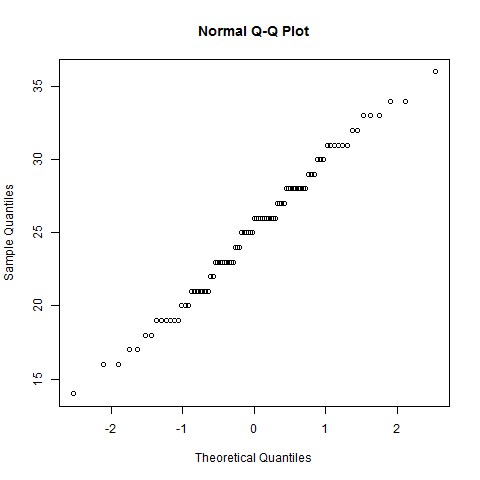
\includegraphics[scale=.33]{QQSci.png}
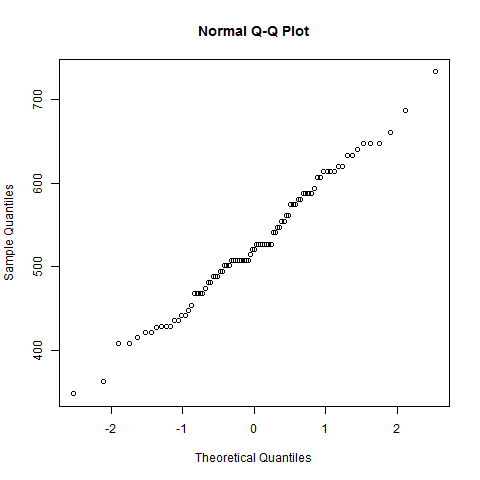
\includegraphics[scale=.33]{QQSoc.png}
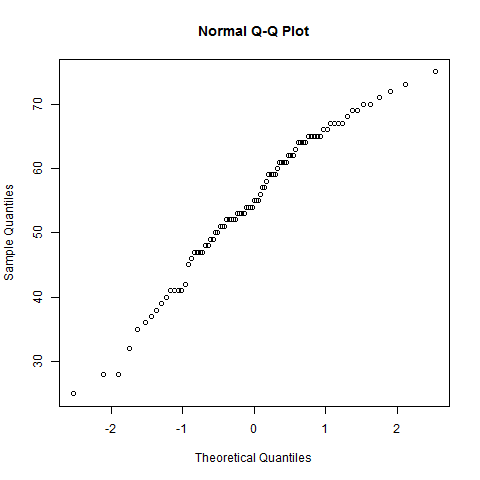
\includegraphics[scale=.33]{QQVerb.png}
\end{center}
With Science, on the left, Social Science and History in the center, and Verbal on the right.\\
The scatter plots of the paired variables are,
\begin{center}
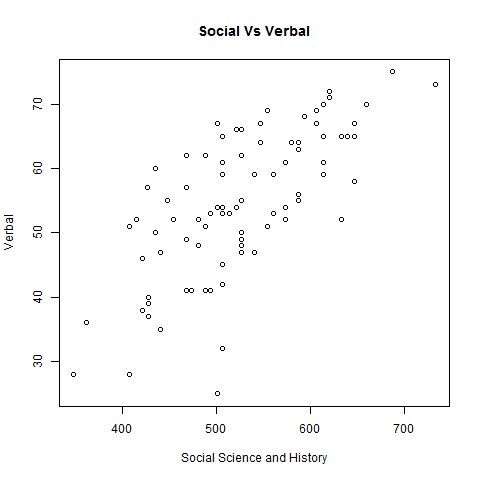
\includegraphics[scale=.33]{SocialvHistory.png}
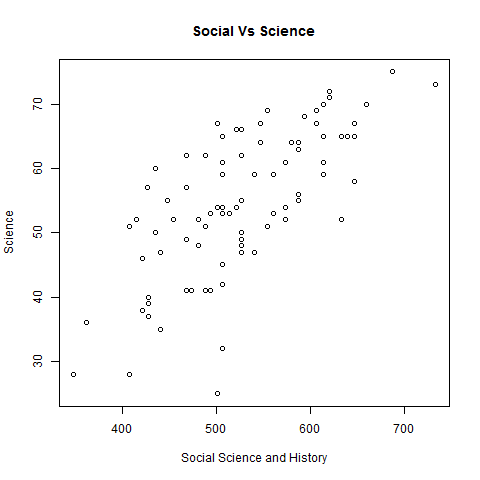
\includegraphics[scale=.33]{SocialvScience.png}
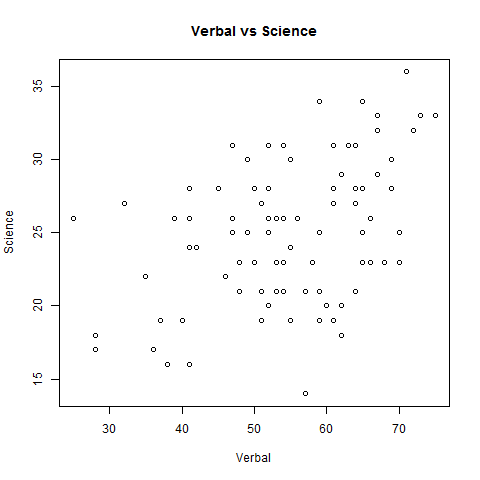
\includegraphics[scale=.33]{VerbalvScience.png}
\end{center}
We see that the QQ plots for the data are indeed straight, as we would expect from normal data, and when we consider the scatter plots of the data, we see that there is not a strong correlation between any two of the variables. This is a good sign of independence for the data.
\end{enumerate}
\item[5.22]\hfill\\
\begin{enumerate}
\item We consider the QQ plots of the non-adjusted data,
\begin{center}
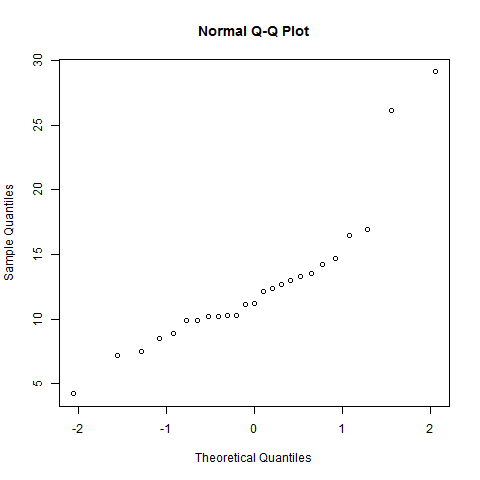
\includegraphics[scale=.33]{QQFuel.png}
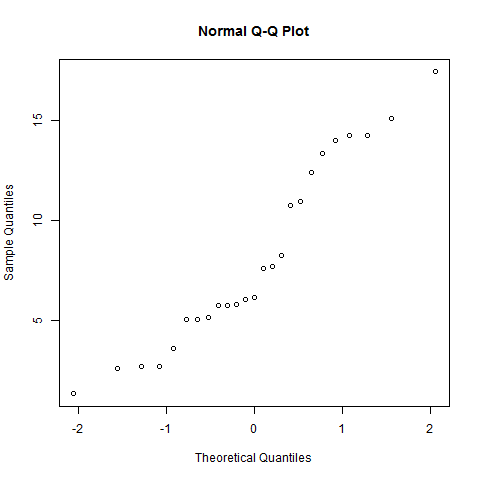
\includegraphics[scale=.33]{QQRepair.png}
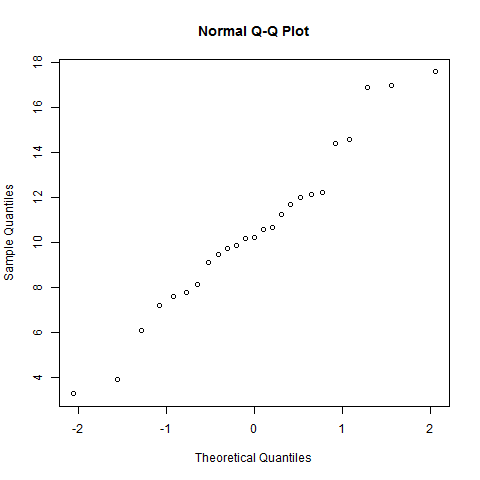
\includegraphics[scale=.33]{QQCapital.png}
\end{center}
And the paired scatter plots,
\begin{center}
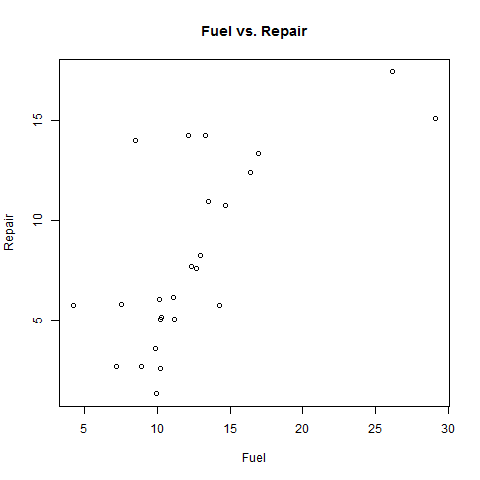
\includegraphics[scale=.33]{FuelvRepair.png}
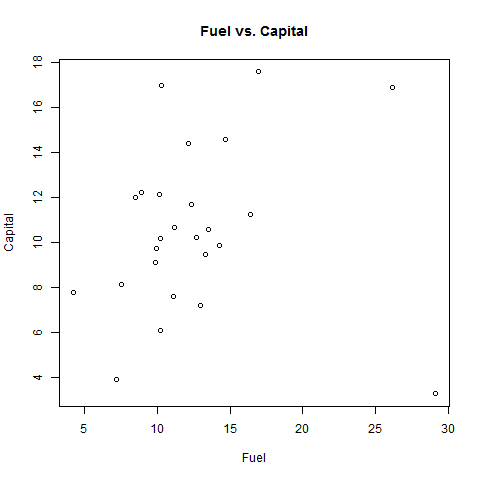
\includegraphics[scale=.33]{FuelvCapital.png}
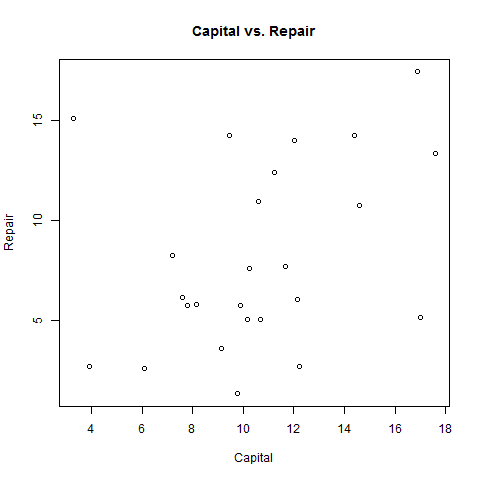
\includegraphics[scale=.33]{CapitalvRepair.png}
\end{center}
We see that the outliers show up in both of these visualizations. We remove the data, and compute again,
\begin{center}
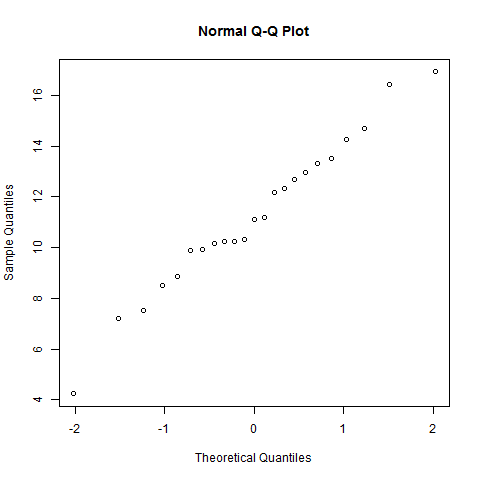
\includegraphics[scale=.33]{QQFuelOut.png}
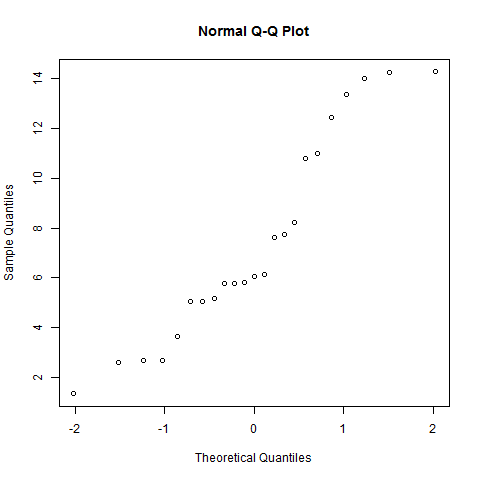
\includegraphics[scale=.33]{QQRepairOut.png}
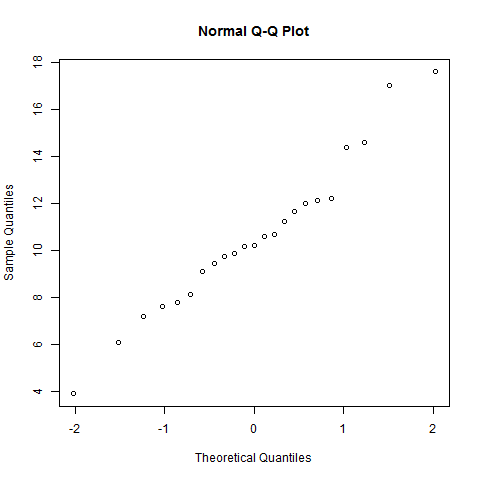
\includegraphics[scale=.33]{QQCapitalOut.png}
\end{center}
And the paired scatter plots,
\begin{center}

\includegraphics[scale=.33]{FuelvRepairOut.png}

\includegraphics[scale=.33]{FuelvCapitalOut.png}

\includegraphics[scale=.33]{CapitalvRepairOut.png}
\end{center}
With the removal of the outliers, we see that the QQ plots straighten out, and are more likely to be normally distributed.
\item As before, we construct the 95\% CI's with both methods,
\begin{align*}
I_{Fuel} &= [9.063887,\ 13.43437]\\
I_{Repair} &= [4.682705,\ 10.23034]\\
I_{Capital} &= [8.41293,\ 12.75577]\\
B_{Fuel} &=[9.478298,\ 13.01996]\\
B_{Repair} &=[5.208732,\ 9.704311]\\
B_{Capital} &=[8.824719,\ 12.34398]
\end{align*}
Again, we see that the Bonferroni intervals fall within the traditional 95\% intervals, as we would expect.
\end{enumerate}
\item[5.23]\hfill\\
We consider the QQ plots of the data below,
\begin{center}
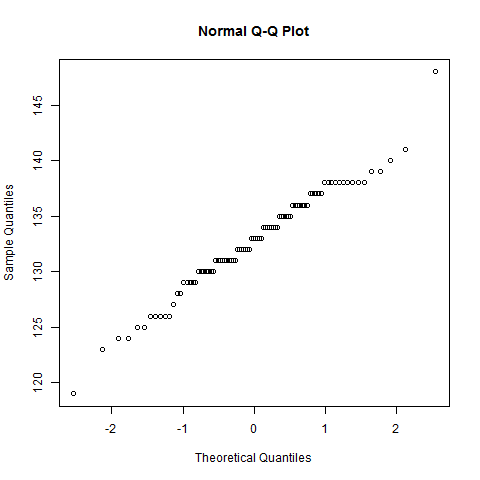
\includegraphics[scale=.25]{QQMaxB.png}
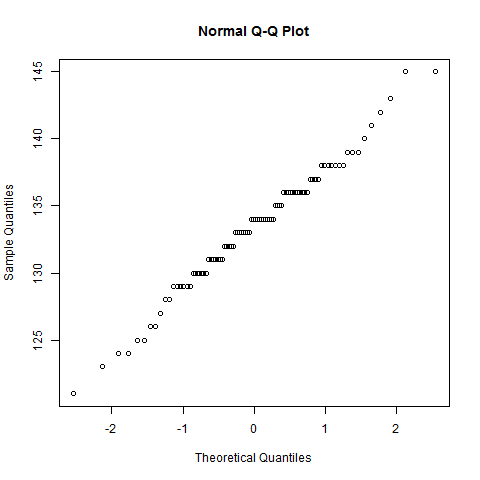
\includegraphics[scale=.25]{QQBasH.png}
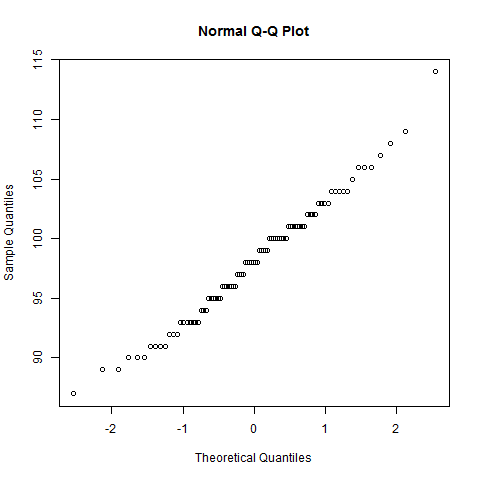
\includegraphics[scale=.25]{QQBasL.png}
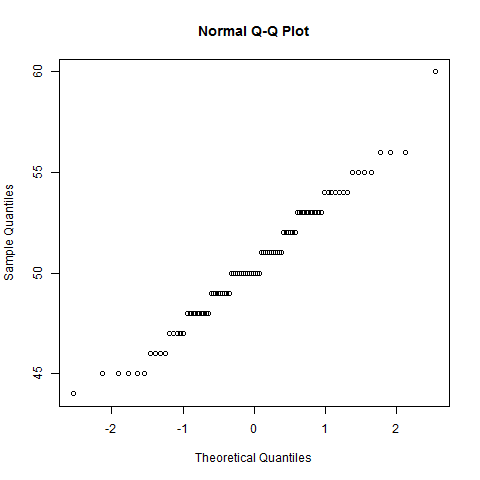
\includegraphics[scale=.25]{QQNasH.png}
\end{center}
With the variables in order from left to right, MaxBreath, BasHeight, BasLength, NasHeight. We also compute the Chi-Square plot,
\begin{center}
\includegraphics[scale=1]{5Chi.png}
\end{center}
We see that all of the QQ plots and the Chi Square plot are linear, so we see that the data is likely normal.\\
We now construct both types of confidence intervals for comparison,
\begin{align*}
I_{MaxBreath} &= [131.159,\ 134.3077]\\
I_{BasHeight} &= [131.7886,\ 134.9448]\\
I_{BasLength} &= [96.35668,\ 99.8211]\\
I_{NasHeight} &= [48.71224,\ 52.17665]\\
B_{MaxBreath} &=[31.4801,\ 133.9866]\\
B_{BasHeight} &=[132.1104,\ 134.6229]\\
B_{BasLength} &=[96.70994,\ 99.46784]\\
B_{NasHeight} &=[49.06549,\ 51.8234]
\end{align*}
Again, we see that the Bonferroni intervals fall within the traditional 95\% intervals, as we would expect.
\end{description}
\end{document}
